\documentclass[conference]{IEEEtran}
\IEEEoverridecommandlockouts

\usepackage{cite}
\usepackage{amsmath,amssymb,amsfonts}
\usepackage{algorithmic}
\usepackage{graphicx}
\usepackage{textcomp}
\usepackage{xcolor}
\usepackage{authblk}
\def\BibTeX{{\rm B\kern-.05em{\sc i\kern-.025em b}\kern-.08em
    T\kern-.1667em\lower.7ex\hbox{E}\kern-.125emX}}
\begin{document}

\title{DNA Sequence Classification for Detection of Plasmid Fragments}

\author[1]{Mehnaz Yunus}
\author[1]{Sharanya Kamath}
\author[1]{Nagaratna B Chittaragi}
\author[1]{Shashidhar G Koolagudi}
\affil[1]{
Department of Computer Science and Engineering, National Institute of Technology Karnataka
\authorcr Email: {\tt \{16co124mehnaz, 16co140.sharanya\}@nitk.edu.in}\vspace{1.5ex}
}

\maketitle

\begin{abstract}
DNA classification is the problem of identifying the functionality of genes using only the sequence information (ATGTGT...) automatically. To figure out the objectives of various proteins and genes, sequence classification has appealed an abundance of consideration in genomic studies. Plasmids are round or straight dual-stranded DNA molecules which are proficient of self-governing duplication and are interchangeable between various bacteria. In silico approaches for forecasting of dna aspects like dna sequence strands are undoubtedly varied for plasmid and chromosomal variants, accordingly establishing a requirement for distinguishment of plasmid and chromosomal sequences in given genomes. 

We developed a machine learning model for discrimination between plasmid-derived and chromosome-derived sequences.

\end{abstract}

\begin{IEEEkeywords}
DNA sequence classification, bi-directional lstm, recurrent neural networks, plasmids
\end{IEEEkeywords}

\section{Introduction}
Sequence classification has a wide bound of actual utilizations. In genomic studies, segregating protein arrangements into extant classes is used to determine the behaviours of an emerging protein. In health-studies, segregating ECG (cardiac rates) time series lets us know if the information is of a fit individual or of a sufferer of cardiac ailments. In intrusion detection, the arrangement of an end users’ setup admittance actions is surveyed to catch peculiar natures. For data retrieval, segregating files into various topic sections has appealed a huge amount of considerations. Other fascinating examples include segregating log arrangements of queries to recognize artificial intelligence machines from humans, and classifying transaction chain information in an investment firm for the desire of opposing wealth fraud.
\newline

Usually, sequences are defined as a systematized register of actions. Actions can be defined as a symbolic assessment, a complex data type, a numerical real assessment,  or a vector of real assessments. We acknowledge sequence information to be a sequence of DNA structure made up of four amino acids T, G, C, A as well as a segment of DNA, such as ACGGTAGC sequence. In prevailing sequence classification, all individual sequences are correlated with a single classification label. The entire sequence is accessible to a predefined classifier. The classification takes place after the classifier.
\newline

Coming era sequencing technologies produce huge amounts of genomic sequence data in the form of RNA or DNA patterns. Study of genomic patterns is vital in avoiding the growth of bacteria, as well as deployed to detect disease during the beginning stages. 

Innovative methods such as Deep Neural Networks (DNN) are in the process of adaptation for sequential dilemmas such as pattern recognition, gene expression inference, and predicting the harmful nature of genetic variants.\cite{danq}

\section{Literature Survey}
An efficient model that forecasts the action of noncoding DNA has huge amount of advantages for both translational studies and traditional science, the reason being that more than 97\% of our DNA sequence is non-coding and 92\% of ailment related varieties exist within such areas.
\newline

Conventionally, studying DNA patterns include motif recognition motifs or phylogenetic analogy with previously known DNA patterns. Segregating an unfamiliar DNA pattern depends primarily on extraction and engineering of features with the help of existing data with annotation from experts. Past researches have shown that word embedding vector representations of trigram form of amino-acid are possible to be trained on massive sequences of protein data.\cite{survey} Ensuing vector representations preserved existing bio-relationships. These representations were used as features for classification of protein families.
\newline

Overcoming this void among annotated and sequenced DNA patterns is essential. For this, in silico methods have been thought of thoroughly. These methods primarily us machine learning approaches like SVM (Support Vector Machines) and ANN  (Artificial Neural Networks).\cite{deeprnn} Other in silico methods are established on the study of physiochemical virtues, amino-acid predispositions, and statistical ability. Equivalent approaches are possible to be unified to form meta-classifiers, which use the outcomes of auxiliary classifiers to compose their augmented classifications.
\newline

Lately, implementation of deep-neural-networks over protein patterns has allowed improved knowledge of complicated relationships amongst structures, arrangements and actions of amino-acids. These networks have at least 2 hidden layers. This implementation has also led to the progress in the accurateness of protein disorder prediction, pair-wise connection prediction, and solvent-accessible-surface area prediction.\cite{danq} Nonetheless, known deep-learning approaches, like RNNs and windowbased ANNs, even though efficient at proliferating local faults within pattern neighbours, are inefficient at recognizing non-neighbour interactions among amino-acid residues. These may be structural neighbours, but they are not sequential neighbours.\cite{shortdna} How to assess residue–residue communications is the answer for improving classification and feature engineering, as they are predominated by structural neighbours.
\newline

Non-neighbour dependency problem among could be analysed by the use of a CEF. CEF or constant-error-flow enables memorization of far range communications.This LSTM network contains hidden-layers which are built of memory units containing at least 1 Long-Short-Term-Memory cell. Every network unit is able to either output,give  input to, or forget the CEC or the Constant-Error-Carousel. This carousel ventures through each LSTM unit in the whole sequence. It bridges the entire pattern by substituting as a pillar for memorization, in the front or back direction. LSTM-based neural networks have been fortuitously used for audio and video related dilemmas for which far range dependency is the answer for definite analysis.
\newline

In recent years, neural networks have consistently achieved avant-garde results on tasks such as language analytics. These networks are now being adopted to solve biotechnological problem statements.\cite{deeprnn} Tackling the problem statement of DNA classification is essential because research in this could help us in better understanding of growth of bacteria, viruses, as well as early disease diagnosis. Existing studies show that methods such as clustering algorithms (k-means), k-mer approach, k-nearest neighbours approach, support vector machines, eigen value vector, and random forest correlation are currently applied for prediction of neuro-genomic ailments.\newline

Currently implemented methods for plasmid-chromosomal classification:
\begin{itemize}
    \item Support Vector Machine\newline
    The Support Vector Machine is a machine learning algorithm which has been utilized for biotechnological problems like recognition of protein family members. Due to its state-of-the-art metaphysical infrastructure, it is an appropriate algorithm for improving classification accuracy in language modeling. K-mer based SVM gave an average classification accuracy of 0.871625.\cite{svm}

    \item Random Forest.\newline
    RF classification algorithm for genomic classification makes use of trees that are disciplined based on arbitrary collection of strains as well as genes. Strains with similar incident patterns could get varied contribution scores. This score is an assessment of how essential a strain is to accurately predict a specific gene. Genes that are either existing or non-existing in all queried genes have inconsequential effects to separate genes of varying phenotype. Random Forest gave a classification accuracy of 0.791423.\cite{randomforest}\newline
\end{itemize} 

Approaches mentioned above have no doubt helped in progressing the have obviously facilitated the advancement in the field of biotechnology and feature engineering. Nevertheless, additional research and analysis is direly needed. Nearly every one of the ML approaches suggest a requirement of static vector length input field. But DNA sequences seldom have static lengths, significant variation is expected. In the process of word-vector formation, pattern order data and dependency equations of position are cast away. This data is an extremely integral part of DNA pattern analysis and genome classification. Even though there are researches which try to contain this data as input to the classifiers, the attempt is not easy because of the Although some studies attempted to incorporate this information into the predictors, it is never an easy task due to the inadequate familiarity with DNA sequences.

\section{Problem Description}
We attempt to classify DNA sequences into either plasmid or chromosomal, by learning the features present in the DNA character sequence using LSTM networks.
The various tools, procedures, methodologies and algorithms available for DNA classification are to be analysed  and compared to find the best and most effective. 

A suitable dataset for the purpose is to be found and if not found, one is to be created by manually labelling the fetched tweets.

Improvement of performance of prediction to initial implementation of DNA classification is attempted. The accuracy of prediction of chromosomal or plasmid in the considered dataset by using the trained model is to be analysed and further improvisation of the accuracy is to be attempted.


\section{Methodology}   

\subsection{Workflow}
We start with character level prediction on DNA sequences. Here, we test whether an LSTM model can accurately predict the next character in a DNA sequence, for manufactured sequences. This will show whether the chosen model is suitable for the classification task or not.

To confirm that an LASTM can model the structure within a genomic sequence, we first train a simple character-level LSTM to predict one of the four possible characters given the previous string of characters. If the LSTM does not give the accuracy as expected, then we will have to more carefully tweak our model until we can identify some signal. Moreover, this simpler task will help us to choose an appropriate architecture for our model.  

Once we have empirical evidence that an LSTM can capture the non-random structure within a genome, we explore a sequence classification problem. The DNA classification task into chromosomal and plasmid is carried out next.

\subsection{Dataset}
DNA, protein and genomic sequences have been made available in a lot of public databases, some of them being EMBL Nucleotide Database, NCBI, GenBank.

The two tasks we performed used different datasets.

For character level genome prediction, our baselines were the artificial genomes. Any model that doesn’t achieve results as required on these two genomic sequences will not be used for further experimentation.
Two genomes were prepared:

\begin{itemize}
    \item A length-3000 repeating genome where the repeated unit is AGCTTGAGGC.
    \item A length-3000 random genome.
\end{itemize}
\newline
For binary classification of DNA sequences the dataset used was from the CAMI project and was obtained from NCBI(National Center for Biotechnology Information) archives. It contained E. Coli complete genomes and plasmids. This dataset contains 3000 DNA sequences of length 500, each with a label indicating whether the sequence is plasmid or chromosomal. 

\subsection{Bidirectional LSTM (BLSTM)}
A BLSTM (bi-directional long short-term memory network) is an alternative to an RNN that unifies the outcomes of two RNNs, one handling the pattern from right to left, and one from left to right. As a substitute to basic hidden cells, these two RNNs consist of LSTM memory units, which are network cells that can memorize a value for a random period of time. Long-term dependencies can be detected by BLSTMs and these networks have been efficient for other machine learning usages such as machine translation, human action recognition, speech recognition and phoneme classification. Even though BLSTMs are efficient for modelling sequential information, they have not yet been tested on DNA sequences. \cite{bidirprotein}

\begin{figure}[h]
\centering
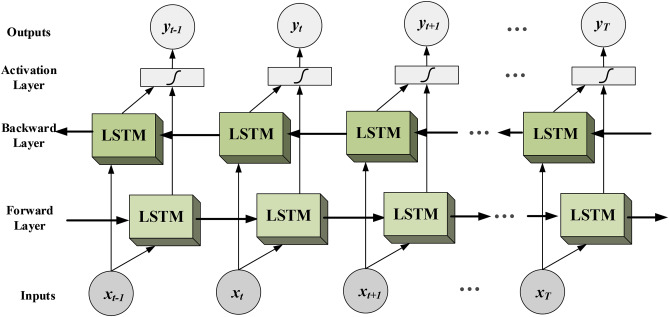
\includegraphics[width=3in]{bidir.jpg}
\DeclareGraphicsExtensions.
\caption{BLSTM}
\label{fig_sim}
\end{figure}

\subsection{Character Level Prediction}
For the character level prediction, an LSTM model with 75 memory cells was used. If this model does not perform as expected on these two genomes, it would point to LSTMs being unable to properly model DNA behaviour\cite{shortrnn}.
\begin{itemize}
    \item Accuracy for repeating genome: 1.0 after 25 epochs
     \item Accuracy for random genome: 0.25 after 25 epochs
(as expected).
\end{itemize}

These experiments showed that an LSTM model may be appropriate for modeling a genomic sequence.



\begin{figure}[h]
\centering
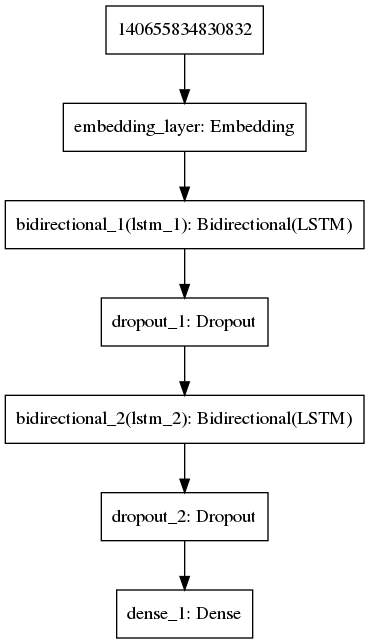
\includegraphics[width=3in]{model.png}
\DeclareGraphicsExtensions.
\caption{Model}
\label{fig_sim}
\end{figure}
% 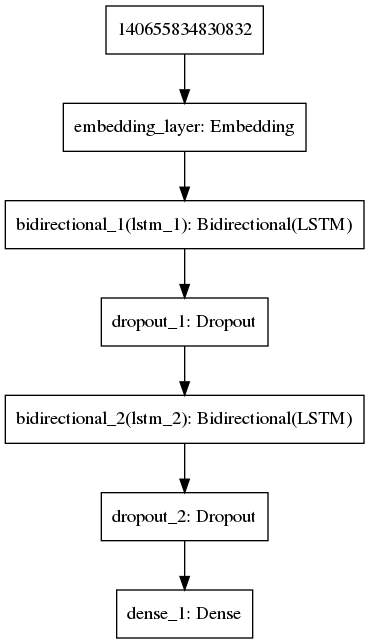
\includegraphics[width=\textwidth]{model.png}

\subsection{Sequence classification}

The  model used contains six layers. The input goes to an embedding layer in which the ACGT sequence is embedded to numerical data. This is followed by 2 sets of bidirectional layer and dropout layer which randomly drops out 20\% of the neurons. Finally there is a fully connected layers which produces the final output. One-hot encoding is used in the input layer for encoding the protein sequences in the input layer.
The dependency connections among sub sequences are withdrawn by the bidirectional LSTMs. Superiority of every transitional obscured term from bidirectional LSTM is taken into account for better handling of the long dimension of DNA patterns. Additional detailed dependency data are possible to be comprehended into the obscured terms by using BLSTM. The transitional obscured terms which are thus obtained are attached with the next fully connected layer. Memorization units in a single LSTM cell abstract various stages of the dependency data. Because of this reason, the dense layer is expected to properly assign weights to the dependency connections abstracted from various units. The outcomes of the final fully connected layer are integrated into a single vector, called a feature vector. This is then fed as input to the final output layer to predict the class.
This neural network enables the capturing of both long term and short term dependency data of pseudo proteins by collecting data from each transitional obscured term of the BLSTM.\newline

We determined the rate of learning in the early stages of training. It was found that the network did not converge with learning rates greater than 0.0001. The step-by-step learning-rate decaying method was employed for reducing the learning rate by 1\% in all epochs. For this, we initialised the learning rate at 0.0001. The rate was then decreased to 5*10\^-5 in 100 epochs. The model was thus able to imbibe fine details as the training progressed. A softmax function is finally used to squeeze the two outputs of the network through a probability distribution.
\newline

We used 5-fold cross-validation for this problem. We partition the original sample to five same-sized subsamples. One of these five subsamples is kept aside as the validation data which is used for testing the model, and the left-over 4 sub-samples are used for training. This process, called cross-validation, is then done five times, with each of the five sub-samples used once as the validation data in rotation. The average of  the five results is then taken to give a single estimation. The leverage of this approach over replicated arbitrary subsampling is that all conclusions are deployed for validation and training both, and each conclusion is deployed only once for validation.

\section{Results and Discussion}
Classifier outputs can be categorized as the following based on sample label: TruePositive(TP), TrueNegative(TN), FalsePositive(FP) and FalseNegative(FN).\newline
Sensitivity (Se=TP/(TP+FN)) and Specificity (Sp=TN/(TN+FP)) are known as performance measuring metrics for two-class classification. The first metric, sensitivity lets us know the capability of the model to accurately distribute the input data within the positive class. The second metric, specificity lets us know the capability of the model to accurately distribute the input data within the negative class. The combination of sensitivity and specificity gives us accuracy(Acc=(Se+Sp)/2).
\newline

The results of the character level prediction fully match the expected results, giving 1.0 for the repeated sequence and 0.25 for the random sequence. We thus proceeded to the next task.
\newline

For the DNA classification, performance is assessed through two-class label analysis. Raw prediction values are also used for this. A softmax function is used to obtain the the prediction probabilities as the final output of the network. The raw probability is converted to discrete labels by comparing with a threshold which is already calculated. The loss on the train dataset decreases as the number of epochs decreases, as expected, and achieves a minimum value of 0.29. The maximum an average validation accuracy obtained were 0.89 and 0.729 respectively.
The graphs for the same are shown in figures 2 and 3.
\newline


\begin{figure}[h]
\centering
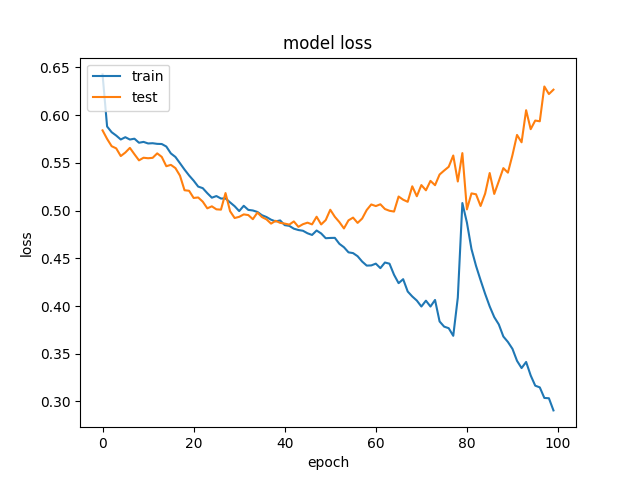
\includegraphics[width=3in]{loss.png}
\DeclareGraphicsExtensions.
\caption{Loss}
\label{fig_sim}
\end{figure}

\begin{figure}[h]
\centering
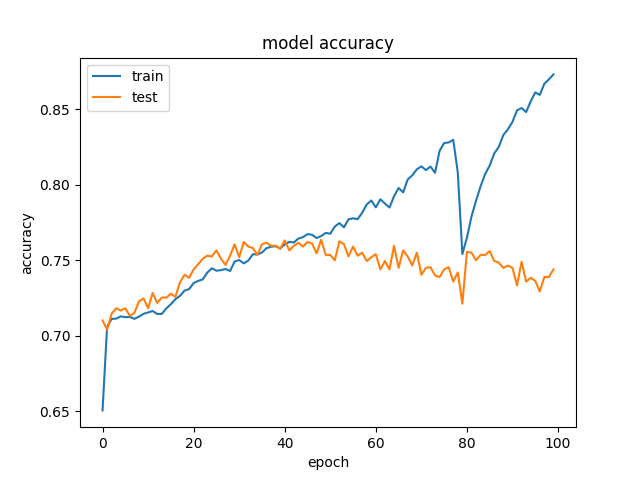
\includegraphics[width=3in]{accuracy.png}
\DeclareGraphicsExtensions.
\caption{Accuracy}
\label{fig_sim}
\end{figure}

\section{Conclusion}
From the preliminary experiments, we were able to deduce that LSTM models are suitable to model DNA sequences effectively. Proceeding to the DNA classification, we developed an LSTM based architecture to classify given DNA sequences into plasmid or chromosomal. The architecture gives an accuracy of 0.89 which performs better than other models used for the same task, such as support vector machine and random forest classifier.

\section{Future interests}
There are several possibilities for future interests. First, we can endeavor to broaden the model to process genetic variants and then predict their functional ramifications. Second, we can use a completely recurrent model so that it can handle sequences of discretionary length, for example, entire chromosome sequences, to produce outputs which are sequential.\newline

Right now, our model can only process sequences which have a fixed length with unchanging outputs. A completely recurrent model can further our effort to study genetic variants. This would help us analyze the long-term implications of the same.\newline

Secondly, we can attempt incorporating more data to test on longer sequences. Fine-tuning hyperparameters, for example, changing the count of layers, increasing the hidden layers, and testing different activation functions can also be tried for increasing accuracy.\newline


\begin{thebibliography}{10}
\bibitem{shortdna} A deep learning approach to pattern
recognition for short DNA sequences, Akosua Busia, George E. Dahl, Clara Fannjiang, June 22 2018.

\bibitem{deeprnn} Deep Recurrent Neural Network for Protein Function Prediction from Sequence, Xueliang Liu, Cornell University, 28 Jan 2017.

\bibitem{deepcg} DeepCpG: accurate prediction of single-cell
DNA methylation states using deep learning, Christof Angermueller, Heather J. Lee, Wolf Reik and Oliver Stegle, Genome Biology (2017)

\bibitem{bidirprotein} Improving protein disorder prediction by deep
bidirectional long short-term memory recurrent neural networks
Jack Hanson, Yuedong Yang, Kuldip Paliwal and Yaoqi Zhou, Oxford, October 26, 2016.

\bibitem{danq} Daniel Quang and Xiaohui Xie. Danq: a hybrid convolutional and recurrent deep neural network for quantifying the function of DNA sequences. bioRxiv, page 032821, 2015.

\bibitem{randomforest} Genotype-phenotype matching analysis of 38 Lactococcus lactisstrains using random forest methods,Jumamurat R Bayjanov, Marjo JC Starrenburg, Marijke R van der Sijde,
BMC Microbiology 2013.

\bibitem{newdna} Qingda Zhou, Qingshan Jiang, Dan Wei, "A new method for classification in DNA sequence", Computer Science \& Education (ICCSE) 2011 6th International Conference on, pp. 218-221, 2011.

\bibitem{survey} A Brief Survey on Sequence Classification, Zhengzheng Xing, Jian Pei, Eamonn Keogh, ACM SIGKDD Explorations Newsletter, Volume 12 Issue 1, June 2010

\bibitem{plasmids} In Silico Detection and Typing of Plasmids,  Alessandra Carattoli, a Ea Zankari.

\bibitem{svm} Gene identification using a support vector machine for ORF classification, Lutz Krause, Alice C. McHardy  Tim W. Nattkemper.

\end{thebibliography}
\vspace{12pt}
\end{document}
